\documentclass[12pt, twoside]{article}
\usepackage[francais]{babel}
\usepackage[T1]{fontenc}
\usepackage[latin1]{inputenc}
\usepackage[left=5mm, right=5mm, top=5mm, bottom=5mm]{geometry}
\usepackage{float}
\usepackage{graphicx}
\usepackage{array}
\usepackage{multirow}
\usepackage{amsmath,amssymb,mathrsfs}
\usepackage{textcomp}
\pagestyle{empty}
\usepackage{soul}
\usepackage{eurosym}


\begin{document} 



\begin{flushleft}
NOM PRENOM: \ldots \ldots \ldots \ldots \ldots \ldots \ldots \ldots \ldots
 \end{flushleft}


\begin{center}
{\fbox{$6^{e}\ldots$ \qquad \qquad \textbf{\Large{Devoir surveill� 1 }}
\qquad \qquad 10/10/2013}}
\end{center}


\bigskip
 
 
 \begin{center}
 \begin{tabular}{|c|c|c|c|}
 \hline
 \quad & un peu & beaucoup & pas du tout \\
 \hline
 J'ai r�vis� & \quad & \quad & \quad \\
 
 \hline
 J'ai r�ussi &  & & \\
 \hline
 
 \end{tabular}

\bigskip

\begin{tabular}{|c|c|c|c|}
\hline

\quad & acquis & en cours d'acquisition & non acquis \\
\hline
Lire et utiliser des donn�es dans un tableau & \quad & \quad & \quad \\
\hline
Interpr�ter des r�sultats & \quad & \quad & \quad \\
\hline
Choisir la bonne op�ration & \quad & \quad & \quad \\
\hline

\end{tabular}
 \end{center}


\bigskip

\bigskip


\textit{Les exercices 3 et 6 sont � faire sur la photocopie. Tout le reste se
fait sur votre feuille pr�par�e.}

\bigskip


\bigskip



\ul{\textbf{Exercice 1:}} \textit{(4 points)}

\begin{tabular}{cc}
\begin{minipage}{11cm}
\begin{enumerate}
  \item Quels sont les fleuves traversant la Chine?
  \item Quel est le plus long fleuve du monde? Quelle est sa longueur?
  \item Quel fleuve a son embouchure en mer Jaune?
  \item Pr�ciser tout ce que le tableau permet de savoir sur le fleuve Amour.
\end{enumerate}
\end{minipage}
&
\begin{minipage}{7cm}
\begin{center}
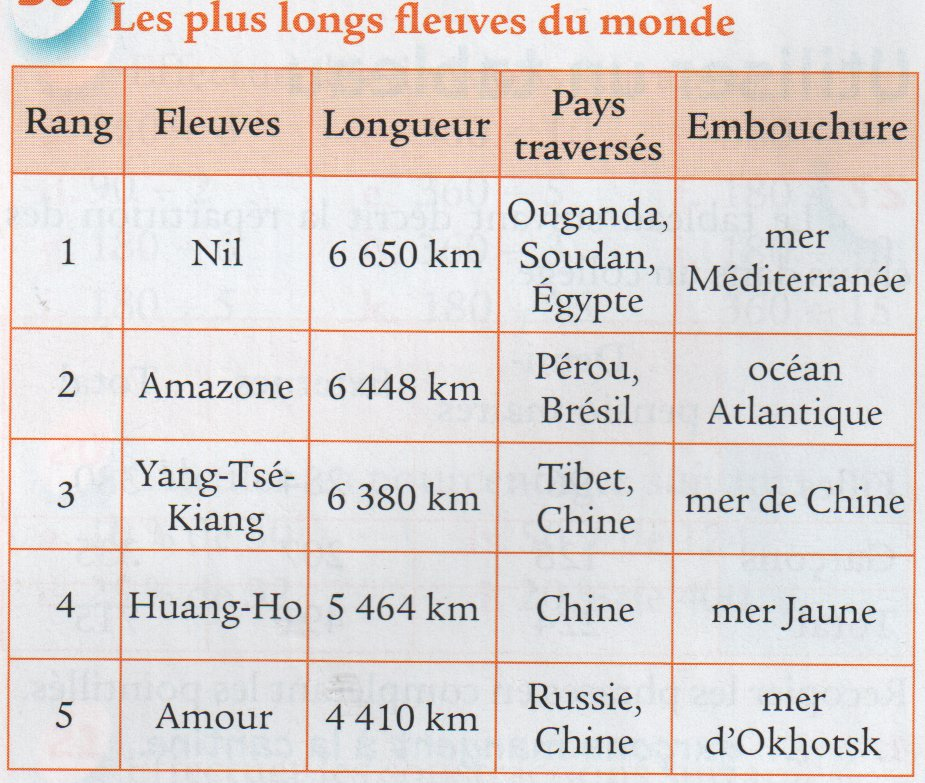
\includegraphics[width=6cm]{images/fleuves.jpg}
\end{center}
\end{minipage}
\end{tabular}

\bigskip

\ul{\textbf{Exercice 2:}} \textit{(4 points)}

\begin{tabular}{cc}
\begin{minipage}{11cm}
\begin{enumerate}
  \item \begin{enumerate}
          \item Combien la France comptait-elle d'habitants en 1900?
          \item Combien la France comptait-elle d'habitants en 1960?
          \item Combien la France comptait-elle d'habitants en 2002?
\end{enumerate}

\item En quelle ann�e la population fran�aise a-t-elle  atteint 50 millions?
\end{enumerate}
\end{minipage}
&
\begin{minipage}{80mm}
\begin{center}
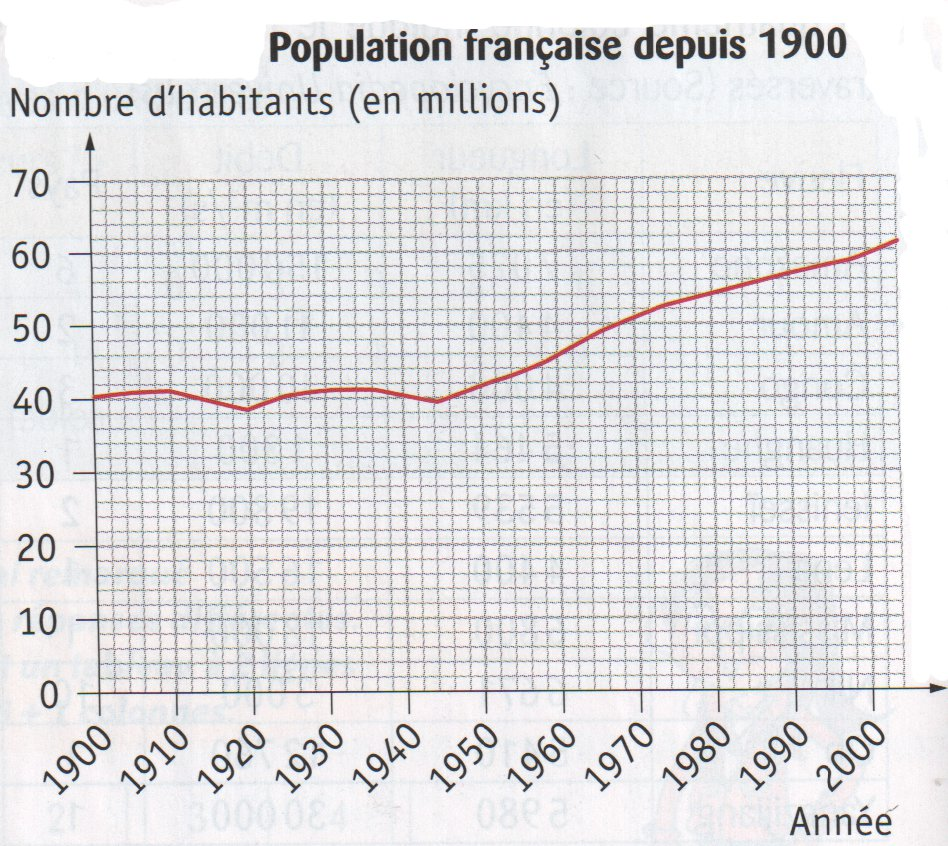
\includegraphics[width=8cm]{images/population.jpg}
\end{center}
\end{minipage}
\end{tabular}

\bigskip

\ul{\textbf{Exercice 3:}} \textit{(4 points)}

\begin{tabular}{cc}
\begin{minipage}{10cm}
Le tableau ci-contre donne la r�partition des musiciens de l'orchestre du
coll�ge Albert Camus.

\begin{enumerate}
  \item Combien y a-t-il de fl�tistes dans cet orchestre? 
  
  \ldots \ldots \ldots \ldots \ldots \ldots \ldots \ldots \ldots \ldots \ldots
  \ldots \ldots \ldots \ldots
  \item Quel est le nombre de gar�ons guitaristes?
  
  \ldots \ldots \ldots \ldots \ldots \ldots \ldots \ldots \ldots \ldots  \ldots
  \ldots \ldots \ldots \ldots
  \item Compl�ter le tableau. \ul{Ecrire les calculs} � c�t� du tableau.
\end{enumerate}
\end{minipage}
&
\begin{minipage}{8cm}

\begin{center}
\begin{tabular}{|c|c|c|c|}
\hline
\quad & Filles & Gar�ons & Total \\
\hline
Fl�tiste & 3 & \qquad & 5 \\
\hline
Guitariste &  \quad & 9 & 10 \\
\hline
Violoniste & 2 & \quad & 6 \\
\hline
Saxophoniste & \quad & 2 & \quad \\
\hline
Total & 6 & \quad & \quad \\
\hline
\end{tabular}
\end{center}
\end{minipage}
\end{tabular}




\bigskip


\ul{\textbf{Exercice 4:}} \textit{(4 points)}


\begin{tabular}{cc}
\begin{minipage}{9cm}
\begin{enumerate}
  \item Fatima entre dans la gare de Tournan � 19h29.
  
   \begin{enumerate}
     \item  Elle souhaite aller � Mortcerf. Quel train peut-elle prendre?
     \item De combien de temps a-t-elle rat� le train pr�c�dent?
     \item Combien de temps va-t-elle attendre le train suivant?
   \end{enumerate}
   
   \item C�dric a pris le train 98C. Il a rendez-vous devant la gare de
   Mouroux � 13h50. Sera-t-il � l'heure � son rendez-vous? Expliquer.
\end{enumerate}
\end{minipage}
&
\begin{minipage}{9cm}
\begin{center}
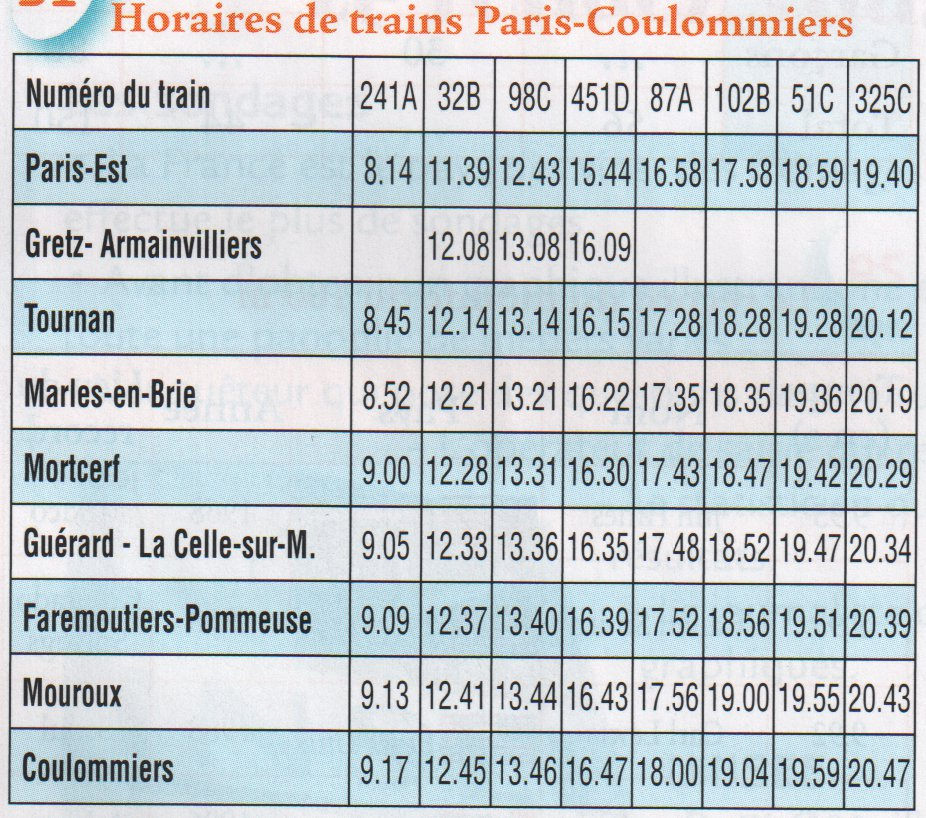
\includegraphics[width=9cm]{images/train.jpg}
\end{center}
\end{minipage}
\end{tabular}

\bigskip



\ul{\textbf{Exercice 5:}} \textit{(2 points)}

\enskip

Voici les 22 notes d'une classe de sixi�me � une �valuation de math�matiques:

\enskip

\begin{center}
\fbox{\begin{minipage}{15cm}
 15; 8; 16; 12; 11; 9; 13; 4; 18; 4; 11; 10; 10; 20; 2; 11; 7; 15; 10; 18; 12;
 14
      \end{minipage}}

\end{center}

\enskip


Construire un tableau indiquant pour chaque note le nombre d'�l�ves ayant
eu cette note (on classera les notes par ordre croissant).


\bigskip

\ul{\textbf{Exercice 6:}} \textit{(2 points)}

\enskip

 Compl�ter le tableau � double entr�e ci-dessous.

\enskip

\begin{tabular}{cc}
\begin{minipage}{9cm}
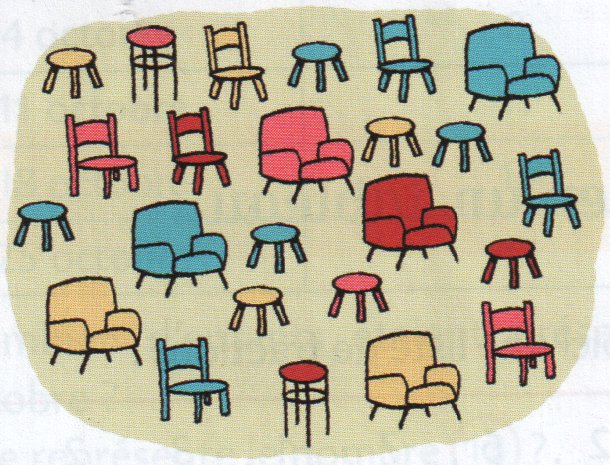
\includegraphics[width=8cm]{images/chaises.jpg}
\end{minipage}
&
\begin{minipage}{9cm}
\begin{center}
\begin{tabular}{|c|c|c|c|}
\hline

\quad \qquad \qquad & fauteuil & chaise & tabouret \\
\quad \qquad \qquad & \quad  &  \quad & \quad   \\


\hline


3 pieds \qquad  & \quad & \quad & \quad \\

\hline

4 pieds \qquad  & \quad & \quad & \quad \\

\hline
\end{tabular}
\end{center}
\end{minipage}
\end{tabular}






\end{document}